\documentclass[a4paper, titlepage]{article}

\usepackage[ngerman]{babel}
\usepackage[utf8]{inputenc}
\usepackage[T1]{fontenc}
\usepackage{lmodern}
\usepackage{csquotes}
\usepackage{hyperref}
\usepackage{graphicx}
\usepackage{svg}
\usepackage{listings}
\usepackage{xcolor}

\definecolor{bluekeywords}{rgb}{0,0,1}
\definecolor{greencomments}{rgb}{0,0.5,0}
\definecolor{redstrings}{rgb}{0.64,0.08,0.08}
\definecolor{xmlcomments}{rgb}{0.5,0.5,0.5}
\definecolor{types}{rgb}{0.17,0.57,0.68}

\usepackage{listings}
\lstset{language=[Sharp]C,
captionpos=b,
%numbers=left, %Nummerierung
%numberstyle=\tiny, % kleine Zeilennummern
frame=lines, % Oberhalb und unterhalb des Listings ist eine Linie
showspaces=false,
showtabs=false,
breaklines=true,
showstringspaces=false,
breakatwhitespace=true,
escapeinside={(*@}{@*)},
commentstyle=\color{greencomments},
morekeywords={partial, var, value, get, set},
keywordstyle=\color{bluekeywords},
stringstyle=\color{redstrings},
basicstyle=\ttfamily\small,
}

\graphicspath{ {./images/}}

\title{Echoes}
\author{Damien Flury, Tim Hess}
\date{30. November 2018}

\begin{document}
    \maketitle
    \tableofcontents
    \newpage
    
    \section{Auftrag}
    Unser Auftrag besteht darin, eine Applikation mit Datenbankanbindung zu entwickeln. Technologien
    können frei gewählt werden.
    \section{Idee}
    Unsere Idee ist die Entwicklung einer Webapplikation für die Planung von Hausaufgaben
    und Prüfungen. 
    \section{Projektbeschreibung}
    Die Webapplikation soll die Verwaltung verschiedener Klassen mit Schülern ermöglichen.
    Man soll einen Account erstellen, Hausaufgaben und Prüfungen zu einer Klasse hinzufügen
    und diese auch als erledigt markieren können. Auf die jeweiligen Hausaufgaben einer Klasse
    haben alle zugehörigen Schüler Zugriff und können diese lesen. Ob sie Aufträge auch bearbeiten
    können, ist noch nicht endgültig entschieden. Momentan planen wir, die Bearbeitung für den Ersteller
    des Auftrags zu ermöglichen, aber nicht für die anderen Schüler. Man soll Aufträge kommentieren
    können.
    \section{Technologien}
    Für die Webapplikation verwenden wir verschiedene Frameworks. Serverseitig bieten wir
    eine REST API mit ASP.NET Core an, Clientseitig konsumieren wir diese API mit dem Single
    Page Application (SPA) Framework Angular.
    \subsection{Backend}
    \begin{itemize}
        \item ASP.NET Core 2.1
        \item C\# 7.3
        \item MariaDB
        \item Entity Framework Core
    \end{itemize}
    \subsection{Frontend}
    \begin{itemize}
    \item Angular 7
    \item Typescript
    \item Bootstrap 4
    \end{itemize}

    \section{Datenbank und konzeptionelles Datenmodell}
    Wie in Abbildung \ref{erd} ersichtlich, verwenden wir eine relationale Datenbank. Für die Anbindung an die Applikation
    verwenden wir Entity Framework Core. Die Tabelle \emph{ApplicationUser}
    ist für das Login zuständig und besitzt eine 1-1 Beziehung mit \emph{Student}.
    Jeder Student gehört einer oder keiner \emph{Class} (Schulklasse) an. Eine Schulklasse besitzt
    keine oder mehrere \emph{Assignments}, also Aufträge. Die Tabelle \emph{StudentAssignment}
    bietet die Möglichkeit, die Hausaufgaben, welche bereits erledigt wurden,
    zu markieren.
    \begin{figure}
        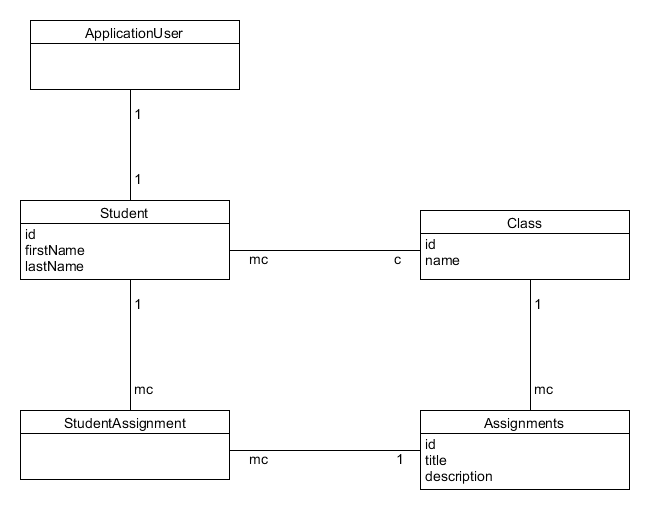
\includegraphics[width=\textwidth]{uml}
        \caption{Entity Relationship Diagram (ERD)}
        \label{erd}
    \end{figure}

    \begin{figure}
        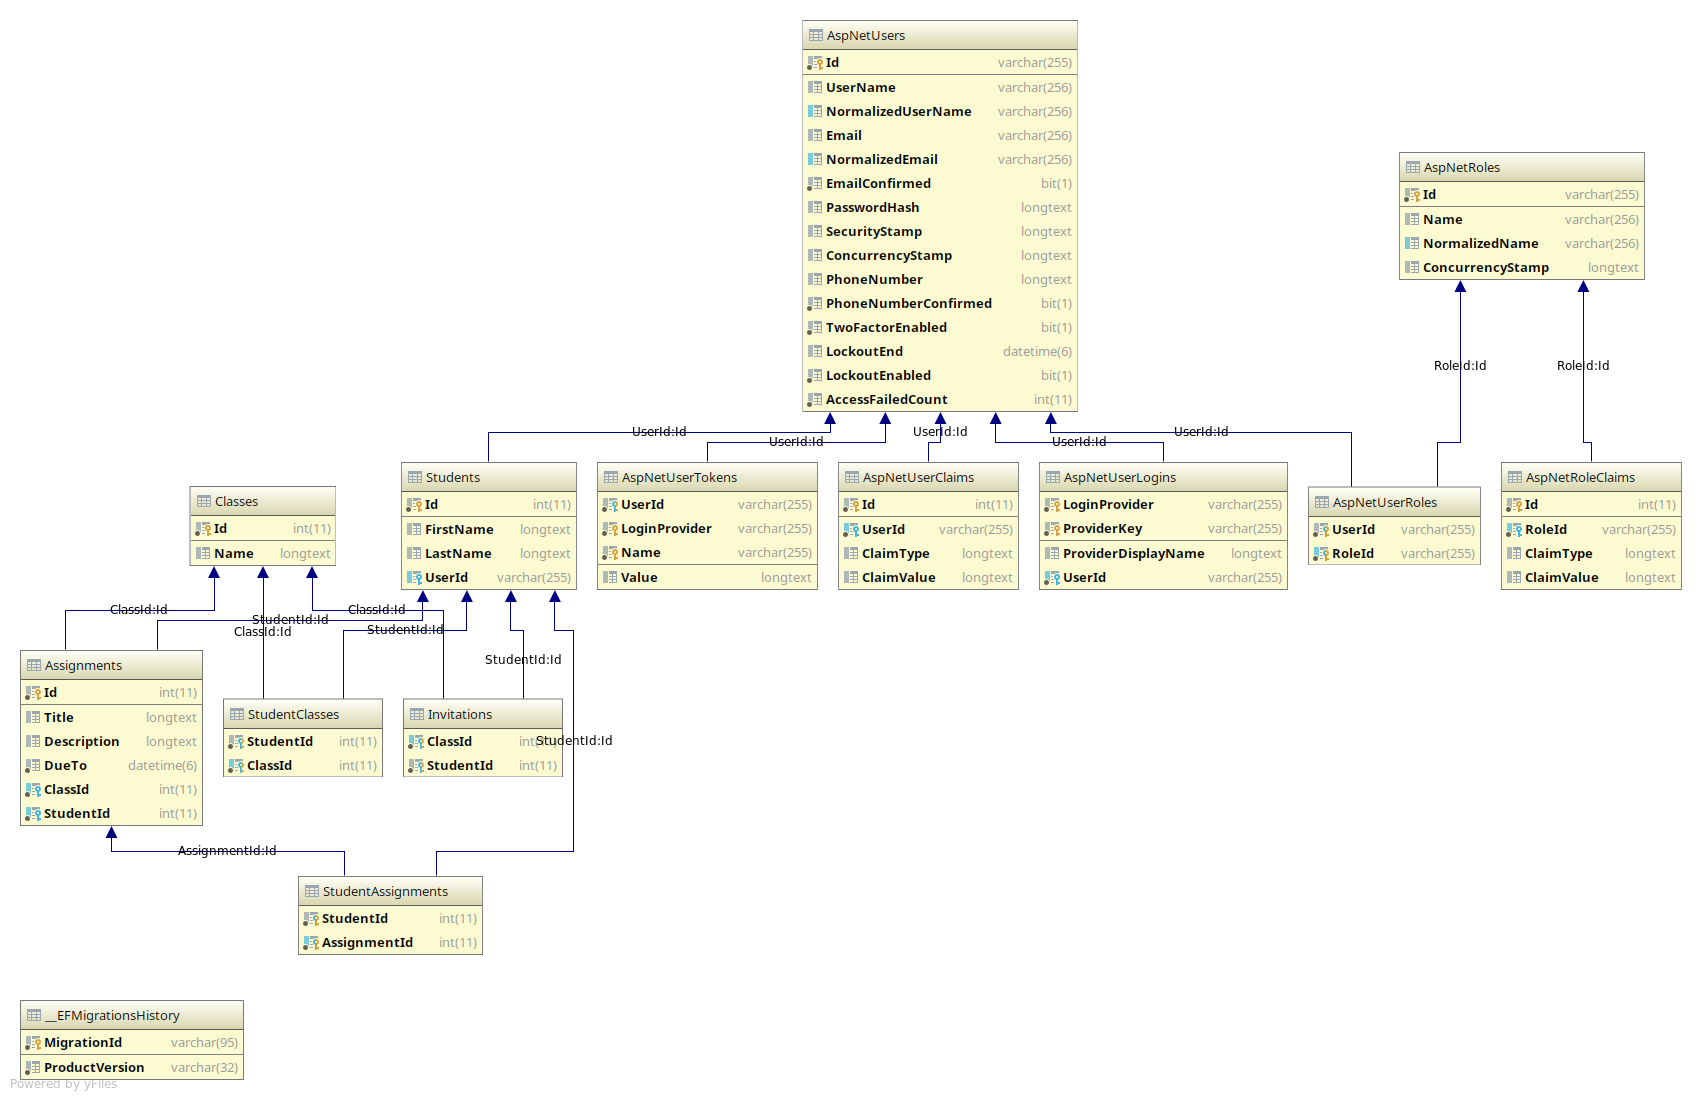
\includegraphics[width=\textwidth]{uml2}
        \caption{Entity Relationship Diagram (Generated)}
    \end{figure}

    \section{REST API}
    Wir verwenden das platformunabhängige Framework ASP.NET Core für die Erstellung einer REST-API.
    Der Datenbankzugriff läuft über Entity Framework Core. Die Tabellen werden automatisch aus dem Model
    generiert. Es wird zunächst eine Datenbankmigration erstellt, welche danach auf die Datenbank mit dem
    \emph{update}-Command auf die Datenbank angewandt werden kann.
    \begin{verbatim}
        $ dotnet ef migrations add Initial
        $ dotnet ef database update
    \end{verbatim}
    ASP.NET Core verwendet standardmässig das MVC-Pattern. Somit haben wir Controller, welche die API-Schnittstellen
    darstellen (Siehe Listing \ref{controller}).

    \begin{figure*}
    \begin{lstlisting}[caption=Controller, label=controller, language=C]
[Route("api/[controller]")]
[ApiController]
[Authorize]
public class AssignmentsController : ControllerBase
{
    [HttpGet]
    public ActionResult<IEnumerable<Assignment>> Get()
        => Ok(GetAll());
}
    \end{lstlisting}
\end{figure*}

    Die Datenbank-Aufrufe erfolgen über \emph{LINQ} (Language Integrated Query), eine Abstraktion, um
    SQL-Statements in C\# selbst zu schreiben. Dies erfolgt entweder über die Lambda-Syntax (Siehe Listing \ref{lambda}), oder über die Query-Syntax
    (Siehe Listing \ref{query}). Das Mapping auf die Objekte erfolgt automatisch.

    \begin{figure*}
    \begin{lstlisting}[caption=Lambda-Syntax, label=lambda]
var assignments = GetAll()
    .Where(assignment => assignment.DueTo < DateTime.Now)
    .OrderBy(assignment => assignment.DueTo);
    \end{lstlisting}

    \begin{lstlisting}[caption=Query-Syntax, label=query]
var assignments = from assignment in GetAll()
    where assignment.DueTo < DateTime.Now
    orderby assignment.DueTo
    select assignment;
    \end{lstlisting}
\end{figure*}


    \section{App}
    Für das Frontend verwenden wir Angular, ein Single Page Application (SPA) Framework. Dies ist Component-Based
    und arbeitet viel mit Property-Binding. Für die API-Aufrufe verwenden wir die Klasse \emph{HttpClient} (Siehe 
    Listing \ref{httpclient}).

    \begin{figure*}
        
    \begin{lstlisting}[language=java,caption=HttpClient, label=httpclient]
export class AssignmentsService {
    constructor(private http: HttpClientService) {}
    
    getAssignments(): Observable<Assignment[]> {
        return this.http
            .get<Assignment[]>('/api/Assignments');
    }
} 

    \end{lstlisting}
    \end{figure*}

    \section{Endprodukt}
    Bis jetzt hat Echoes einige nützliche Funktionen für Schüler und Lehrer. Sowohl Schüler als auch Lehrer können sogenannte Assignments 
    in jeder Klasse erstellen und ein Datum dazusetzen. Diese Assignments werden danach auf dem Tab \emph{My Assignments} angezeigt. 
    Wenn das Datum des Assignments abgelaufen ist, wird es im Subtab \emph{Inactive} angezeigt. Diese Assignments werden zusätzlich nur angezeigt, 
    wenn der User sich in der Klasse befindet, in der das Assignment erstellt wurde. Klassen kann man sehr einfach erstellen und gewisse Schüler 
    mit ihrer eingegebenen Email-Adresse zur Klasse einladen. Wird ein Schüler eingeladen, kann er die Einladung im \emph{Invitations} Tab 
    finden und akzeptieren.
    
    \section{Zukünftige Erweiterungen und Updates}
    Wir haben definitiv noch weitere Ideen, die wir bei Echoes einbauen können. Da jetzt der grundlegende Baustein des Projektes gelegt ist, kann man noch viele zukünftige Updates darauf aufbauen und erweitern. Wir planten, dass Schüler abhaken können, ob sie ein Assignment schon fertiggestellt haben und dass diese Liste von Schülern für den Ersteller des Assignments sichtbar ist.
    

    % \begin{figure}
    %     
\includegraphics[width=\textwidth]{angular}
    %     \caption{Angular}
    % \end{figure}
    % \begin{figure}
    %     
\includegraphics[width=\textwidth]{csharp}
    %     \caption{C\#}
    % \end{figure}

    \newpage
  
\end{document}
